%(BEGIN_QUESTION)
% Copyright 2006, Tony R. Kuphaldt, released under the Creative Commons Attribution License (v 1.0)
% This means you may do almost anything with this work of mine, so long as you give me proper credit

Et type ``T'' termoelement består av ulike metaller: kobber (Cu) og Constantan (C). Kobber er et grunnstoff, mens Constantan er en legering av kobber og nikkel. Termoelementtabeller fra instrumentleverandører oppgir ofte måleskjøtspenning ved ulike temperaturer med antatt referanseskjøt på 32$^{o}$ F, eller 0$^{o}$ C (frysepunktet til rent vann). Bruk en slik tabell og bestem utgangsspenning for type ``T'' termoelement av massiv 16 AWG ved følgende prosesstemperaturer:

$$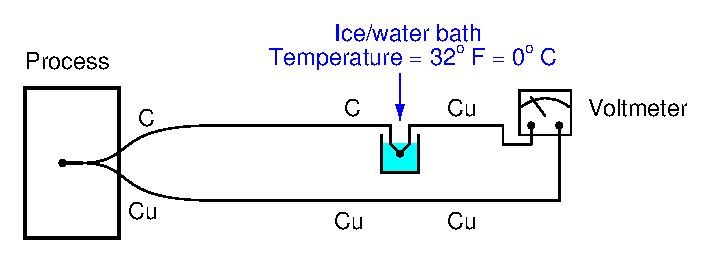
\includegraphics[width=15.5cm]{i00367x01.eps}$$

\begin{itemize}
\item{} $T_{process}$ = 350$^{o}$ F; voltmeterspenning = ???
\item{} $T_{process}$ = $-$65$^{o}$ F; voltmeterspenning = ???
\item{} $T_{process}$ = 32$^{o}$ F; voltmeterspenning = ???
\item{} $T_{process}$ = 100$^{o}$ C; voltmeterspenning = ???
\end{itemize}

\vskip 10pt

Bestem også standard fargekoder for type T-termoelementledning:

\begin{itemize}
\item{} Positiv leder:
\item{} Negativ leder:
\item{} Kappe for termoelementkvalitet:
\item{} Kappe for forlengelseskvalitet:
\end{itemize}

\vskip 20pt \vbox{\hrule \hbox{\strut \vrule{} {\bf Forslag til sokratisk diskusjon} \vrule} \hrule}

\begin{itemize}
\item{} Forklar hvorfor is-vannbad brukes ved referanseskjøten. Forklar også hvorfor bare én av referanseskjøtforbindelsene er i badet, mens den andre (Cu/Cu) ikke er det.
\item{} Hvis is-vannblandingen smelter helt og temperaturen stiger, hvordan påvirkes målenøyaktigheten? Gir det \textit{nullpunktskift}, \textit{spanskift} eller endret \textit{linearitet}?
\end{itemize}

\underbar{file i00367}
%(END_QUESTION)





%(BEGIN_ANSWER)

(Fra ITS-90 termoelementtabell:)

\begin{itemize}
\item{} $T_{process}$ = 350$^{o}$ F; voltmeterspenning = 8.064 mV
\item{} $T_{process}$ = $-$65$^{o}$ F; voltmeterspenning = $-$1.950 mV
\item{} $T_{process}$ = 32$^{o}$ F; voltmeterspenning = 0 mV
\item{} $T_{process}$ = 100$^{o}$ C; voltmeterspenning = 4.279 mV
\end{itemize}

\vskip 10pt


Fargekoder:

\begin{itemize}
\item{} Positiv leder: {\it Blå}
\item{} Negativ leder: {\it Rød}
\item{} Kappe for termoelementkvalitet: {\it Brun}
\item{} Kappe for forlengelseskvalitet: {\it Blå}
\end{itemize}

Den siste temperaturen var et ``lurespørsmål''! Du måtte enten konvertere 100$^{o}$ C til Fahrenheit (212$^{o}$ F), eller slå opp i tabell indeksert i Celsius.

\vskip 10pt

Ledningsdimensjonen (16 AWG) er overflødig informasjon, lagt inn for å utfordre studenten til å vurdere om opplysninger er relevante for løsning av oppgaven.

%(END_ANSWER)





%(BEGIN_NOTES)


%INDEX% Measurement, temperature: thermocouple (type T)

%(END_NOTES)
